\documentclass[./project-report/src/latex/project-report.tex]{subfiles}

\begin{document}

\maketitle

\section{Analysis}

\subsection{About}

Artificial Intelligence mimics human cognition in order to perform tasks and learn from them, Machine Learning is a subfield of Artificial Intelligence that uses 
algorithms trained on data to produce models (trained programs) and Deep Learning is a subfield of Machine Learning that uses Artificial Neural Networks, a process of 
learning from data inspired by the human brain. Artificial Neural Networks can be trained to learn a vast number of problems, such as Image Recognition, and have uses 
across multiple fields, such as medical imaging in hospitals. This project is an investigation into how Artificial Neural Networks work, the effects of changing their 
parameters and their applications in Image Recognition. To achieve this, I will derive and research all theory behind the project, using sources such as IBM's online 
research, and develop Neural Networks from first principles without the use of any third-party Machine Learning libraries. I then will implement the Artificial Neural 
Networks in Image Recognition, by creating trained models and will allow for experimentation of the parameters of each model to allow for comparisons between each 
model's performances, via a Graphical User Interface.

\subsection{Interview TODO}

In order to gain a better foundation for my investigation, I presented my prototype code and interviewed the head of Artificial Intelligence at Cambridge Consultants 
for input on what they would like to see in my project, these were their responses:

% Use google doc file of qs

% Notes:
% - ReLu stops vanishing gradients
% - Validation set
%   - Monitors how well network is predicting, to see when network becomes overtrained
% - Progress bar
% - cfar-10 dataset
% - To expand dataset, take sections of images
% - Save a trained network to load later
% - Transfer functions
% - Maybe CNNs
% - Jupyter notebook for technical solutions
% - Browse through more of results
%   - Show images predicted correct
%   - Show images predicted wrong
%   - Show images where prediction is close between muliple classes
% - Play around with size of training dataset
%   - Graph showing performance against increase in training data

\begin{itemize}
    \item Q:""

          A:""
\end{itemize}

\subsection{Project Objectives}

\begin{itemize}
    \item Learn how Artificial Neural Networks work and develop them from first principles
    \item Implement the Artificial Neural Networks by creating trained models on image datasets
    \begin{itemize}
        \item Allow use of Graphics Cards for faster training
        \item Store trained weights with sqlite
    \end{itemize}
    \item Develop a Graphical User Interface
    \begin{itemize}
        \item Provide controls for parameters of models
        \item Display and compare the results each models' predictions
    \end{itemize}
\end{itemize}

\subsection{Theory behind Artificial Neural Networks}

From an abstract perspective, Artificial Neural Networks are inspired by how the human mind works, by consisting of layers 'neurons' all interconnected via 
different links, each with their own strength. By adjusting these links, Artificial Neural Networks can be trained to take in an input and give its best 
prediction as an output.
\vspace{5mm}

\subsubsection{Structure}

\begin{figure}[h!]
\centering
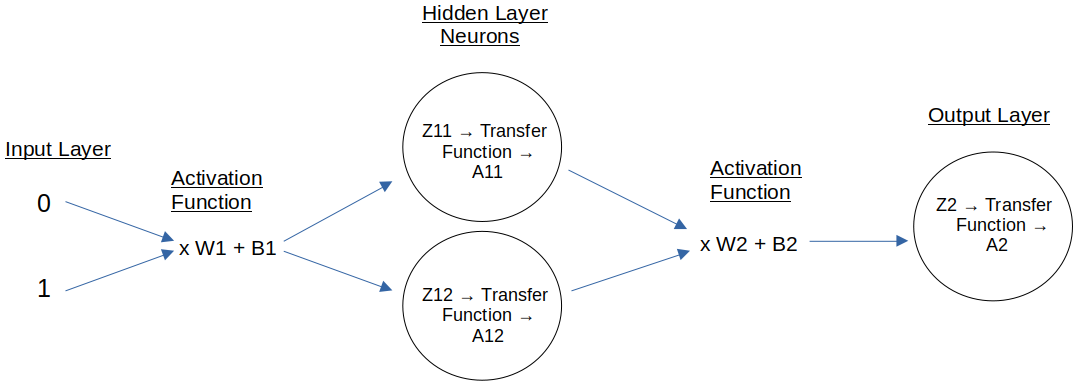
\includegraphics[width=1\textwidth]{./project-report/src/images/shallow-ann-diagram.png}
\caption{This shows an Artificial Neural Network with one single hidden layer and is known as a Shallow Neural Netwok.}
\end{figure}

I have focused on Feed-Forward Artificial Neural Networks, where values are entered to the input layer and passed forwards repetitively to the next layer until 
reaching the output layer. Within this, I have learnt two types of Feed-Forward Artificial Neural Networks: Perceptron Artifical Neural Networks, that contain no 
hidden layers and are best at learning more linear patterns and Multi-Layer Perceptron Artifical Neural Networks, that contain at least one hidden layer, as a result 
increasing the non-linearity in the Artificial Neural Network and allowing it to learn more complex / non-linear problems.

Multi-Layer Perceptron Artificial Neural Networks consist of:

\begin{itemize}
    \item An input layer of input neurons, where the input values are entered.
    \item Hidden layers of hidden neurons.
    \item An output layer of output neurons, which outputs the final prediction.
\end{itemize}

To implement an Artificial Neural Network, matrices are used to represent the layers, where each layer is a matrice of the layer's neuron's values. In 
order to use matrices for this, the following basic theory must be known about them:

\begin{itemize}
    \item When working with two matrices, the number of columns of the 1st matrix must equal the number of rows of the 2nd matrix. And the result will have the same 
          number of rows as the 1st matrix, and the same number of columns as the 2nd matrix. This is important, as the output of one layer must be formatted correctly 
          to be used with the next layer.
    \item In order to multiply matrices, I take the 'dot product' of the matrices, which multiplies the row of one matrice with the column of the other, by multiplying 
          matching members and then summing up.
    \item Transposing a matrix will turn all rows of the matrix into columns and all columns into rows.
    \item A matrix of values can be classified as a rank of Tensors, depending on the number of dimensions of the matrix. (Eg: A 2-dimensional matrix is a Tensor of 
          rank 2)
\end{itemize}

I have focuesd on just using Fully-Connected layers, that will take in input values and apply the following calculations to produce an output of the layer:

\begin{itemize}
    \item An Activation function
    \begin{itemize}
        \item This calculates the dot product of the input matix with a weight matrix, then sums the result with a bias matix
    \end{itemize}
    \item A Transfer function
    \begin{itemize}
        \item This takes the result of the Activation function and transfers it to a suitable output value as well as adding more non-linearity to the Neural Network.
        \item For example, the Sigmoid Transfer function converts the input to a number between zero and one, making it usefull for logistic regression where the output 
              value can be considered as closer to zero or one allowing for a binary classification of predicting zero or one.
    \end{itemize}
\end{itemize}
\vspace{5mm}

\subsubsection{How Artificial Neural Networks learn}
\vspace{5mm}

To train an Artificial Neural Network, the following processes will be carried out for each of a number of training epochs:

\begin{itemize}
    \item Forward Propagation:

    \begin{itemize}
        \item The process of feeding inputs in and getting a prediction (moving forward through the network)
    \end{itemize}

    \item Back Propagation:

    \begin{itemize}
        \item The process of calculating the Loss in the prediction and then adjusting the weights and biases accordingly
        \item I have used Supervised Learning to train the Artificial Neural Networks, where the output prediction of the Artificial Neural Network is compared to the 
              values it should have predicted. With this, I can calculate the Loss value of the prediction (how wrong the prediction is from the actual value).
        \item I then move back through the network and update the weights and biases via Gradient Descent:
        \begin{itemize}
            \item Gradient Descent aims to reduce the Loss value of the prediction to a minimum, by subtracting the rate of change of Loss with respect to the weights
                  biases, multiplied with a learning rate, from the weights/biases.
            \item To calculate the rate of change of Loss with respect to the weights/biases, you must use the following calculus methods:
            \begin{itemize}
                \item Partial Differentiation, in order to differentiate the multi-variable functions, by taking respect to one variable and treating the rest as 
                      constants.
                \item The Chain Rule, where for $y = f(u)$ and $u = g(x)$, $\frac{\partial{y}}{\partial{x}} = \frac{\partial{y}}{\partial{u}} * \frac{\partial{u}}{\partial{x}}$
                \item For a matrice of $f(x)$ values, the matrice of $\frac{\partial{f(x)}}{\partial{x}}$ values is known as the Jacobian matrix
            \end{itemize}
            \item This repetitive process will continue to reduce the Loss to a minimum, if the learning rate is set to an appropriate value
                \begin{figure}[h!]
                \centering
                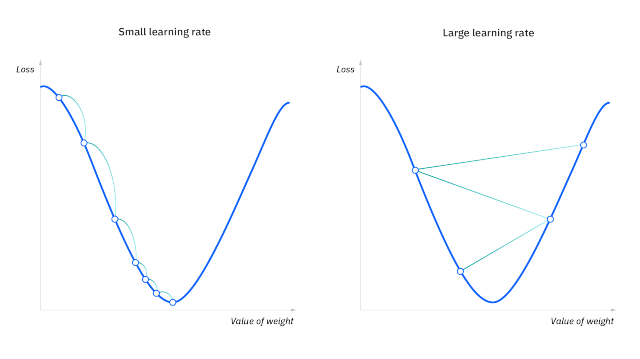
\includegraphics[width=1\textwidth]{./project-report/src/images/gradient-descent.png}
                \caption{Gradient Descent\\
                        sourced from https://www.ibm.com/topics/gradient-descent}
                \end{figure}
            \item However, during backpropagation some issues can occur, such as the following:
            \begin{itemize}
                \item Finding a false local minimum rather than the global minimum of the function
                \item Having an 'Exploding Gradient', where the gradient value grows exponentially to the point of overflow errors
            \end{itemize}
        \end{itemize}
    \end{itemize}
\end{itemize}

\vspace{5mm}
\subsection{Theory Behind Deep Artificial Neural Networks}
\vspace{5mm}

\subsubsection{Setup:}

\begin{figure}[h!]
\centering
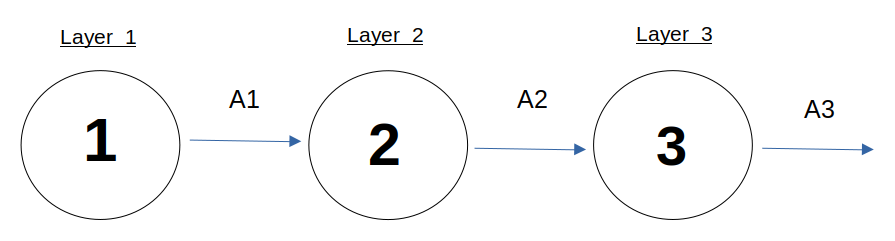
\includegraphics[width=1\textwidth]{./project-report/src/images/deep-ann-diagram.png}
\caption{This shows an abstracted view of an Artificial Neural Network with multiple hidden layers and is known as a Deep Neural Netwok.}
\end{figure}

\begin{itemize}
    \item Where a layer takes the previous layer's output as its input X
    \item Then it applies an Activation function to X to obtain Z, by taking the dot product of X with a weight matrix W, then sums the result with a bias matix B. At 
          first the weights are intialised to random values and the biases are set to zeros.
    \begin{itemize}
        \item $Z = W . X + B$
    \end{itemize}
    \item Then it applies a Transfer function to Z to obtain the layer's output
    \begin{itemize}
        \item For the output layer, the sigmoid function (explained previously) must be used for either for binary classification via logistic regression, or for multi-
              class classification where it predicts the output neuron, and the associated class, that has the highest value between zero and one.
        \begin{itemize}
            \item Where $sigmoid(Z) = \frac{1}{1+e^{-Z}}$
        \end{itemize}
        \item However, for the input layer and the hidden layers, another transfer function known as ReLu (Rectified Linear Unit) can be better suited as it produces a 
              larger value of $\frac{\partial{L}}{\partial{W}}$ for Gradient Descent than Sigmoid, so updates at a quicker rate.
        \begin{itemize}
            \item Where $relu(Z) = max(0, Z)$
        \end{itemize}
    \end{itemize}
\end{itemize}

\subsubsection{Forward Propagation:}

\begin{itemize}
    \item For each epoch the input layer is given a matrix of input values, which are fed through the network to obtain a final prediction A from the output layer.
\end{itemize}

\subsubsection{Back Propagation:}

\begin{itemize}
    \item First the Loss value L is calculated using the following Log-Loss function, which calculates the average difference between A and the value it should have 
          predicted Y. The the average is found by summing the result of the Loss function for each value in the matrix A, then dividing by the number of predictions m, 
          resulting in a Loss value to show how well the network is performing.
    \begin{itemize}
        \item Where $L = -(\frac{1}{m}) * \sum(Y * log(A) + (1-Y) * log(1-A))$ and "log()" is the natural logarithm
    \end{itemize}
    \item I then move back through the network, adjusting the weights and biases via Gradient Descent. For each layer, the weights and biases are updated with the 
          following formulae:
    \begin{itemize}
        \item $W = W - learningRate * \frac{\partial{L}}{\partial{W}}$
        \item $B = B - learningRate * \frac{\partial{L}}{\partial{B}}$
    \end{itemize}
    \item The derivation for Layer 2's $\frac{\partial{L}}{\partial{W}}$ and $\frac{\partial{L}}{\partial{B}}$ can be seen below:
    \begin{itemize}
        \item Functions used so far:
        \begin{enumerate}
            \item $Z = W * X + B$
            \item $A_{relu} = max(0, Z)$
            \item $A_{sigmoid} = \frac{1}{1+e^{-Z}}$
            \item $L = -(\frac{1}{m}) * \sum(Y * log(A) + (1-Y) * log(1-A))$
        \end{enumerate}
        \item $\frac{\partial{L}}{\partial{A2}} = \frac{\partial{L}}{\partial{A3}} * \frac{\partial{A3}}{\partial{Z3}} * \frac{\partial{Z3}}{\partial{A2}}$
              \vspace{1mm}
              \newline
              By using function 1, $\frac{\partial{Z3}}{\partial{A2}} = W3$
              \vspace{1mm}
              \newline
              $=> \frac{\partial{L}}{\partial{A2}} =  \frac{\partial{L}}{\partial{A3}} * \frac{\partial{A3}}{\partial{Z3}} * W3$
        \item $\frac{\partial{L}}{\partial{W2}} = \frac{\partial{L}}{\partial{A2}} * \frac{\partial{A2}}{\partial{Z2}} * \frac{\partial{Z2}}{\partial{W2}}$
              \vspace{1mm}
              \newline
              By using function 1, $\frac{\partial{Z2}}{\partial{W2}} = A1$
              \vspace{1mm}
              \newline
              $=> \frac{\partial{L}}{\partial{W2}} = \frac{\partial{L}}{\partial{A2}} * \frac{\partial{A2}}{\partial{Z2}} * A1$
        \item $\frac{\partial{L}}{\partial{B2}} = \frac{\partial{L}}{\partial{A2}} * \frac{\partial{A2}}{\partial{Z2}} * \frac{\partial{Z2}}{\partial{B2}}$
              \vspace{1mm}
              \newline
              By using function 1, $\frac{\partial{Z2}}{\partial{B2}} = 1$
              \vspace{1mm}
              \newline
              $=> \frac{\partial{L}}{\partial{W2}} = \frac{\partial{L}}{\partial{A2}} * \frac{\partial{A2}}{\partial{Z2}} * 1$
    \end{itemize}
    \item As you can see, when moving back through the network, the $\frac{\partial{L}}{\partial{W}}$ and $\frac{\partial{L}}{\partial{B}}$ of the layer can be 
          calculated with the rate of change of loss with respect to its output, which is calculated by the previous layer using the above formula; the derviative of 
          the layer's transfer function, and the layers input (which in this case is A1)
    \begin{itemize}
        \item Where by using function 2, $\frac{\partial{A_{relu}}}{\partial{Z}} = 1$ when $Z >= 0$ otherwise $\frac{\partial{A_{relu}}}{\partial{Z}} = 0$
        \item Where by using function 3, $\frac{\partial{A_{sigmoid}}}{\partial{Z}} = A * (1 - A)$
    \end{itemize}
    \item At the start of backpropagation, the rate of change of loss with respect to the output layers output has no previous layer's caluculations, so instead it can 
          be found with the derivative of the Log-Loss function, as shown in the following:
    \begin{itemize}
        \item Using function 3, $\frac{\partial{L}}{\partial{A}} = (-\frac{1}{m})(\frac{Y-A}{A * (1-A)})$
    \end{itemize}
\end{itemize}

\subsection{Theory behind training the Neural Networks}

Training an Artificial Neural Network's weights and biases to predict on a dataset, will create a trained model for that dataset, so that it can predict on future 
images inputted. However, training Artificial Neural Networks can involve some problems such as Overfitting, where the trained model learns the patterns of the 
training dataset too well, causing worse prediction on a different test dataset. This can occur when the training dataset does not cover enough situations of inputs 
and the desired outputs (by being too small for example), if the model is trained for too many epochs on the poor dataset and having too many layers in the Neural 
Network. Another problem is Underfitting, where the model has not learnt the patterns of the training dataset well enough, often when it has been trained for too few 
epochs, or when the Neural Network is simple (too linear).

\subsubsection{Datasets}
\vspace{5mm}

\begin{itemize}
    \item MNIST dataset
    \begin{itemize}
        \item The MNIST dataset is a famouse dataset of images of handwritten digits from zero to ten, and is commonly used to test the performance of an Artificial 
              Neural Network.
        \item The dataset consists of 60,000 input images, made up from 28x28 pixels and each pixel has an RGB value from 0 to 255
        \item To format the images into a suitable format to be inputted into the Artificial Neural Networks, each image's matrice of RGB values are 'flattened' into a 
              1 dimensional array of values, where each element is also divided by 255 (the max RGB value) to a number between 0 and 1, to standardize the dataset.
        \item The output dataset is also loaded, where each output for each image is an array, where the index represents the number of the image, by having a 1 in the 
              index that matches the number represented and zeros for all other indexes.
        \item To create a trained Artifical Neural Network model on this dataset, the model will require 10 output neurons (one for each digit), then by using the 
              Sigmoid Transfer function to output a number between one and zero to each neuron, whichever neuron has the highest value is predicted. This is multi-class 
              classification, where the model must predict one of 10 classes (in this case, each class is one of the digits from zero to ten).
    \end{itemize}
    \item Cat dataset
    \begin{itemize}
        \item I will also use a dataset of images sourced from https://github.com/marcopeix, where each image is either a cat or not a cat.
        \item The dataset consists of 209 input images, made up from 64x64 pixels and each pixel has an RGB value from 0 to 255
        \item To format the images into a suitable format to be inputted into the Artificial Neural Networks, each image's matrice of RGB values are 'flattened' into a 
              1 dimensional array of values, where each element is also divided by 255 (the max RGB value) to a number between 0 and 1, to standardize the dataset.
        \item The output dataset is also loaded, and is reshaped into a 1 dimensional array of 1s and 0s, to store the output of each image (1 for cat, 0 for non cat)
        \item To create a trained Artifical Neural Network model on this dataset, the model will require only 1 output neuron, then by using the Sigmoid Transfer 
              function to output a number between one and zero for the neuron, if the neuron's value is closer to 1 it predicts cat, otherwise it predicts not a cat. 
              This is binary classification, where the model must use logistic regression to predict whether it is a cat or not a cat.
    \end{itemize}
    \item XOR dataset
    \begin{itemize}
        \item For experimenting with Artificial Neural Networks, I solve the XOR gate problem, where the Neural Network is fed input pairs of zeros and ones and learns 
              to predict the output of a XOR gate used in circuits.
        \item This takes much less computation time than image datasets, so is usefull for quickly comparing different parameters of a Network.
    \end{itemize}
\end{itemize}

\subsubsection{Theory behind using Graphics Cards to train Artificial Neural Networks}
\vspace{5mm}

Graphics Cards consist of many Tensor cores which are processing units specialiased for matrix operations for calculating the co-ordinates of 3D graphics, however they 
can be used here for operating on the matrices in the network at a much faster speed compared to CPUs. GPUs also include CUDA cores which act as an API to the GPU's 
computing to be used for any operations (in this case training the Artificial Neural Networks).

\end{document}